\section{Results}
\label{sec:results}




% - Figure results.1: Overall error at the end of the trial with unlimited sampling and without weighing by the rarity (1/prob of occurrence) of the class
% - Figure results.2: overall error at the end of the trial with unlimited sampling and with weighing by the rarity of the class
% - Figure results.3: Overall performance when combining limited time and limited sample budgets.
% 
% Different arrival rates and different distributions.

% \begin{figure}[htpd]
% 	\centering
% 	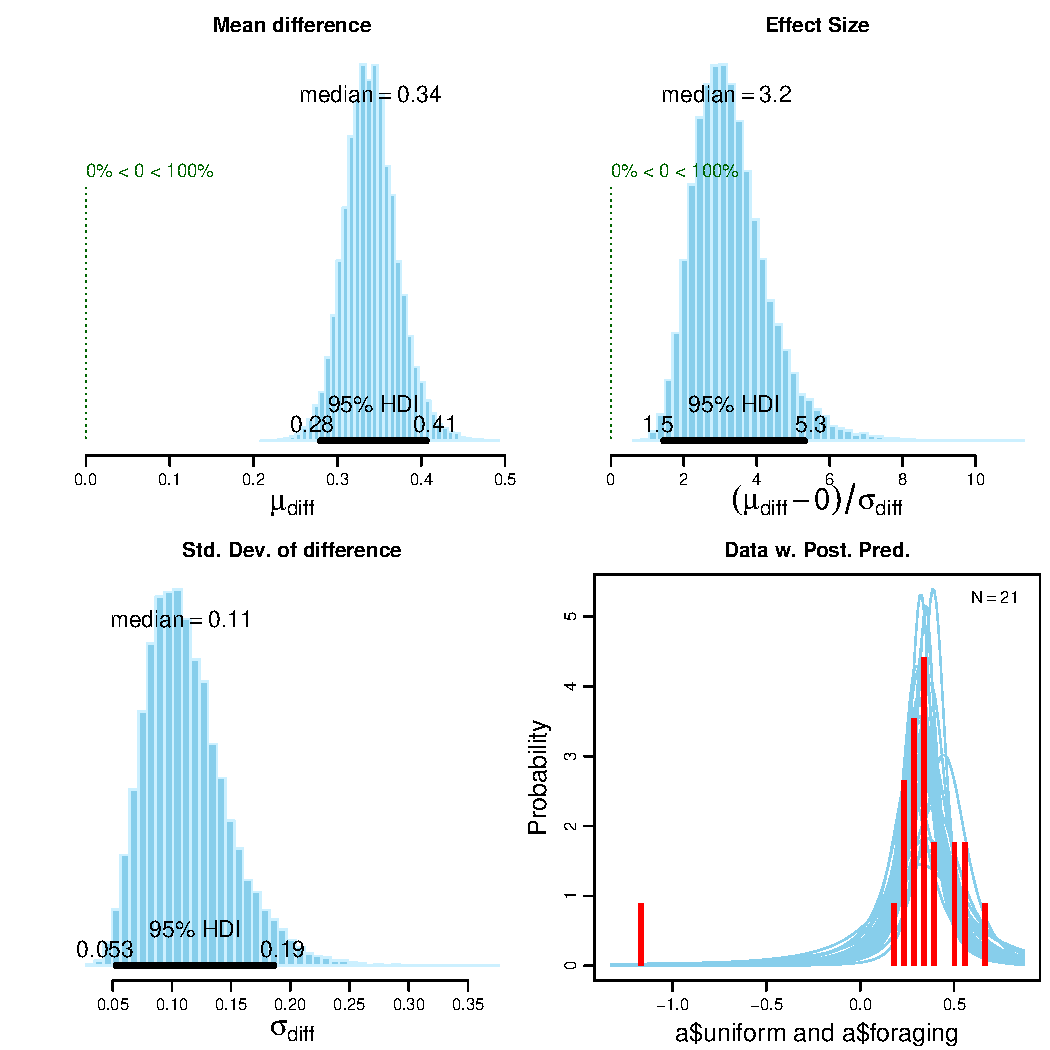
\includegraphics[width=0.8\textwidth]{images/diff-diff.pdf}
% 	\caption{Analysis of the basic scenario with different arrival rates and standard deviations.  We see here the effect size in the reduction in terminal error is 3.2, by Cohen's d measure.  This qualifies as a ``very large'' effect.}
% 	\label{fig:diff-diff}
% \end{figure}
% 

In the experiment the sampling cost is varied from $0.001$ to $150$.  This is a considerable range given the total length of a transect is $1000$ units of time.  When the sampling cost is small, relative to the duration of the transect, the performance of the foraging algorithm is significantly better, as in Figure \ref{fig:err}.  For a portion at the higher end of the spectrum the uniform algorithm outperforms the foraging algorithm.  However at the extreme end the algorithms' performance converges.  

At a sampling cost of 100 time units only ten sampling actions can be taken during a transect that lasts for 1000 time units.  In this case one would expect performance to be limited, as it is difficult to learn much about six different random variables with only ten samples.  


% Accumulated Error 
\begin{figure}[htpd!]
	\centering
	\def\svgwidth{\columnwidth}
	\input{plot_err-vs-cost.pdf_tex}
	\caption{For sampling costs that are small, relative to the duration of the transect, the foraging algorithm presents a significant improvement over the uniform algorithm.  The shaded region covers $1.96\times$ the standard error from the 21 trials, approximating a frequentist 95\% confidence interval, to indicate the variablility of the algorithms' performance.}
	\label{fig:err}
\end{figure}

\subsection{Analysis}

For each of the twenty-one trials the agents were scored on the data they collected when given a fixed sampling cost.  For each sampling cost the performance was tested with a Bayesian paired t-test \cite{baath2014bayesian}.  The paired t-test returns an average difference between the paired trials as well as a 95\% credible interval around that difference.  We accept that the difference is non-zero when the credible interval does not contain 0.  

The test described in \cite{baath2015bayesian} also gives an effect size.  The effect size is the ratio of the mean to the standard deviation of the difference between the paired trials.  This is a variation of Cohen's $d$ value\cite{cohen2013statistical}.  With this number we consider a value greater than 1.3 to be very large, above 0.8 to be significant and below 0.5 to be insignificant.  Table \ref{tbl:ttest} gives the results of the Bayesian paired t-test at different values of sampling cost.

\begin{table}[htpd!]
	\centering
	\begin{tabular}{lccc}
		Cost & Reduction in Error & Credible Interval & Effect Size \\
		\hline
		\textbf{0.001} & \textbf{0.40} & \textbf{[0.34,0.46]} & \textbf{3.5}\\
		\textbf{0.01} & \textbf{0.38} & \textbf{[0.32,0.45]} & \textbf{2.8}\\
		\textbf{0.1} & \textbf{0.24} & \textbf{[0.17,0.31]} & \textbf{1.8}\\
		1.0 & 0.04 & [-0.041,0.11] & 0.24\\
		10.0 & -0.88 & [-1.1,-0.62] & 1.6\\
		100.0 & -0.27 & [-0.53,-0.006] & 0.48\\
		\hline \\
	\end{tabular}
	\caption{Selected datapoints along the graph in Figure \ref{fig:err} along with the associated credible intervals of the difference and the effect size.  Bold rows are case where the foraging algorithm provides a statistically signficant improvement over the uniform sampling algorithm.}
	\label{tbl:ttest}
\end{table}
